% Preprint. Build si.tex first, then main.tex (main.tex reads si.aux for the S-numbers).
% Build: latexmk -pdf main.tex   (refs.bib is generated: python3 manuscript/preprint/make_bib.py)
\documentclass[journal=jacsat,manuscript=article]{achemso}

\usepackage[version=4]{mhchem}
\usepackage{amsmath}
\usepackage{amssymb}
\usepackage{siunitx}
\usepackage{booktabs}
\usepackage{longtable}
\usepackage{xr}
\externaldocument[SI-]{si}  % S-numbers of the Supporting Information (build si.tex first)
\graphicspath{{figs/}{../../figures/}}  % figs/: title-free versions (make_figures.py)
\SectionNumbersOn

% Skeleton marker: renders as a bracketed note so gaps stay visible in the PDF.
\newcommand{\gap}[1]{\textbf{[GAP: #1]}}
\newcommand{\src}[1]{\textsuperscript{\texttt{[#1]}}}  % pointer to the repository file a number comes from

\author{Chan Young Joe}
\affiliation{Independent Researcher, Incheon, Republic of Korea}
\email{ccy5123ccy@gmail.com}

\title{Silent but deadly? Rarely at the nose, usually in memory}

\abbreviations{CFD, computational fluid dynamics; OAV, odour activity value; RANS, Reynolds-averaged Navier--Stokes}
\keywords{flatus, odour dispersion, starting jet, convective boundary layer, Berkson bias, olfactory perception}

\begin{document}

\begin{tocentry}
\gap{TOC graphic: needed only for an ACS journal submission, not for the preprint}
\end{tocentry}

\begin{abstract}
The belief that a silent passage of flatus smells worse than an audible one appears in many languages but has not
been tested. We follow a passage from sound through dispersion to a bystander's memory, using a lip-reed model of the
anal valve, analytic and computational dispersion models and literature observer models. Most releases, 85\%, never
set the valve oscillating. We prove that under linear transport a slower release of the same gas cannot give a higher
peak, in any room or flow. A silent release can win only near the source, where a loud jet is pre-diluted by a
factor set by its exit-to-ambient velocity ratio, the Silencer number. In computational fluid dynamics of seated and
standing people, the warm air rising along the body takes a slow release and lets a fast one pass, so momentum
decides which nose a release reaches. As emitted, a silent passage is the stronger one at a bystander's nose in
\gap{v4} of pairs. A silent passage is noticed only if smelled, and this selection alone can explain the belief: a
remembered silent passage seems the stronger one in \gap{v4} of comparisons. The explanation predicts that releasers
hold the belief less firmly than bystanders and that anosmic people never remember a silent passage.

\end{abstract}

\section{Introduction}
\label{sec:intro}

% Hook (PLAN.md section 2): paraphrase only; no quotation of the verse, no image of the character.
\gap{Hook paragraph.} The nickname of the character Chatur ``Silencer'' Ramalingam in the film \emph{3 Idiots}
\cite{hirani2009} rests on the belief that a silent release is the most offensive; in the film, a mock-Sanskrit verse
ranks releases by sound, from a loud blast down to the silent one, which it declares the deadliest.
An 1811 slang dictionary defines a related term as an escape ``more obvious to the nose than ears'' \cite{grose1811}.

\gap{Paragraph: the conjecture across cultures (32 languages, evidence levels; Figure~\ref{fig:culture}).}

\gap{Paragraph: three meanings of ``silent'' and three comparison bases:
(A) equal mass and composition, (B) as emitted, (C) among noticed events.}

\gap{Paragraph: contributions.}
(i) a mechanistic chain from sound to nose dose;
(ii) two transport theorems that bound what physics can do;
(iii) a selection model that produces the belief from a coin-flip truth;
(iv) a cross-cultural survey.

\section{Definitions and theory}
\label{sec:theory}

\subsection{Deadliness of one passage}
Deadliness is the perceived intensity of the worst single inhalation, $I = k\,\mathrm{OAV}^n$, with the OAV taken as the
flow-weighted mean over one inhalation. Perceived intensity saturates within one sniff
\cite{laing1983,laing1985}, still integrates within it \cite{frasnelli2006}, and the sniff is the unit of olfactory
processing \cite{uchida2003,kepecs2006}; odour-impact regulation also works per breath \cite{schauberger2012}.
Cumulative exposure is a secondary metric.

\subsection{Linear transport (Theorem 1)}
\gap{Statement and proof.} For a passive scalar, $C = G * q$. The time-integrated dose does not depend on the release
history, and a slower release never has a higher peak (Young's inequality), for any Green's function $G$.

\subsection{Loss of release memory (Theorem 2)}
\gap{Statement.} Differences between release modes decay with time and distance; in a closed room both tend to
$M/V_\mathrm{room}$.

\subsection{Where the theorems fail}
Only release momentum and buoyancy break linearity: near-field jet pre-dilution, bounded by the Silencer number
$\mathrm{Si} = u_0/u_h$, and changes of routing, of either sign.

\subsection{Selection (Theorem 3)}
\gap{Statement and proof.} If a passage is remembered when heard ($H$) or smelled ($S$), then
$P(S\mid\neg H, N) = 1$ and $P(S\mid H, N) = P(S\mid H)$, whatever the joint law of $H$ and $S$
\cite{berkson1946,snoep2014}. An observer who notices every passage (the emitter) has no bias.

\section{Methods}
\label{sec:methods}

Every parameter, with its source, range and whether it is measured, derived or assumed, is listed in
Table~\ref{SI-tab:params}. Code and data are archived (Section~\ref{SI-sec:si-data}).

\subsection{Source}
\label{sec:source}
Passage volumes span 17--375\,mL, with a median of 92\,mL \cite{suarez1997}. In the Monte Carlo analysis, volume $V$,
duration $T$ (0.3--20\,s) and effective orifice diameter $d$ (1--8\,mm) are drawn log-uniformly. Neither has been
measured for a passage. The upper bounds come from anorectal physiology: flatus passes during an anal relaxation
lasting $19 \pm 6$\,s \cite{ronholt1999,corsetti2017}, and the mid anal canal widens to about 8\,mm only at balloon
pressures above those that drive flatus \cite{luft2012,sorensen2014,miller1988b}. The lower bounds are assumed.

Sulfur gas concentrations are taken from 87 passages of 16 volunteers \cite{suarez1998}: \ce{H2S}
1.06\,\textmu mol\,L$^{-1}$, methanethiol 0.21\,\textmu mol\,L$^{-1}$ and dimethyl sulfide 0.08\,\textmu mol\,L$^{-1}$.
They vary between passages by a log-normal factor with $\sigma_{\ln} = 1.1$, derived from the reported standard
errors, drawn independently of volume because sulfur concentration does not correlate with passage volume
\cite{suarez1997}. Buoyancy is computed from measured compositions and is signed (Section~\ref{sec:methods-chem}); it
is drawn independently of volume because, across the 16 subjects of ref.~\citenum{suarez1997}, it does not correlate
with mean passage volume (Spearman $-0.15$).

\subsection{Odorant chemistry}
\label{sec:methods-chem}
\emph{Odour activity.} Each sulfur gas contributes an odour activity value (OAV), its mole fraction over its detection
threshold, $\mathrm{OAV}_i = x_i/\theta_i$. The passage's OAV is their sum; we assume additivity and do not model
mixture suppression. We compare two measured compositions:
\begin{itemize}
  \item 87 passages of 16 volunteers \cite{suarez1998}, used throughout the dispersion model;
  \item 28 passages measured by gas chromatography: \ce{H2S} 149, methanethiol 216 and dimethyl sulfide
  144\,nmol\,L$^{-1}$ \cite{tangerman2009}.
\end{itemize}
Three threshold sets bracket the observer: a trained panel \cite{nagata2003}, population geometric means
\cite{amoore1983,wilby1969} and the lowest values in the literature, as compiled in ref.~\citenum{tangerman2009}.

\emph{Removal check.} Zinc acetate precipitates \ce{H2S} and thiols; activated charcoal adsorbs all three gases. For both
treatments, ref.~\citenum{suarez1998} reports the gas concentrations and two judges' ratings before and after. We
predict the rating ratio as $(\mathrm{OAV}_\mathrm{after}/\mathrm{OAV}_\mathrm{before})^n$ with $n = 0.20$--$0.45$
\cite{collins2001}, without fitting.

\emph{Buoyancy.} The reduced gravity $g' = g(\rho_a-\rho_g)/\rho_a$ of each of 16 measured compositions
\cite{suarez1997} is split into a thermal part, $g(1-T_a/T_g)$, for gas at 37\,\textdegree C in air at
22\,\textdegree C, and a compositional part, $g(M_a-M_g)/M_a$, at equal temperature with air at 50\% relative
humidity. The water-vapour content of flatus has not been measured, so we bracket dry and saturated gas.

\emph{Gas-phase and surface losses.} Gas-phase losses use IUPAC rate constants at 298\,K for reaction with OH,
\ce{O3}, \ce{NO3} and Cl \cite{atkinson2004}, with oxidant levels measured in an office: OH
$0.6$--$9.8\times10^{5}$\,cm$^{-3}$ and \ce{O3} 0.7--2.6\,ppb \cite{fiorentino2023}. Two assumed upper cases add OH
$10^6$\,cm$^{-3}$ with \ce{O3} 40\,ppb, and Cl $10^6$\,cm$^{-3}$ during hypochlorite cleaning. No deposition velocity
$v_d$ has been published for these gases on indoor surfaces, so surface loss is bracketed as $k = v_d\,S/V$ with
$S/V = 3$\,m$^{-1}$.

\emph{Dilution in a panel test.} Ref.~\citenum{tangerman2009} reports the lowest source concentration that every panel
member detected when 100\,mL was released below the nose. Divided by a detection threshold, it gives the dilution
between release and nose in that test, which we compare with the breath-averaged dilution of the analytic model.

\subsection{Acoustics}
\label{sec:acoustics}
The anal canal is modelled as a lip reed, a soft-tissue valve that self-oscillates in the flow through it, as the
lips do on a brass instrument. It oscillates when the driving pressure $\tfrac12\rho(u_0/C_\mathrm{d})^2$ exceeds a
threshold $P_\mathrm{th}$ = 0.6--2.5\,kPa (nominal 1.2\,kPa), with discharge coefficient $C_\mathrm{d} = 0.85$. The
closest measured soft-tissue sphincter source, the pharyngo-oesophageal segment of oesophageal speech, sustains
phonation down to 1.1--2.5\,kPa \cite{nagai1993,grolman2007,ng2011}, which bounds the onset from above; lips on a brass
instrument start at about 0.6\,kPa \cite{matteoli2021}. This gives an onset velocity
$u_\mathrm{onset} \approx 42$\,m\,s$^{-1}$ (21--71).

An oscillating valve radiates as a harmonic monopole with harmonics falling by 12\,dB per octave. Its fundamental is
taken as 160\,Hz (60--300\,Hz), between oesophageal speech at 60--150\,Hz \cite{nagai1993,robbins1984,pindzola1989,deschler1999}
and recordings of flatus near 270\,Hz, which are not peer-reviewed. A release counts as \emph{audible} when at least one harmonic exceeds both the ISO 226 hearing threshold
\cite{iso226_2023} and the masked threshold of the background, computed from the critical ratio \cite{hawkins1950}.
Backgrounds range from a 35\,dB(A) living room to a 77\,dB(A) subway car.

\subsection{Analytic dispersion model}
\label{sec:gate0}
Dispersion is modelled in two phases.
\begin{enumerate}
  \item \emph{Near field.} The release behaves as a starting jet. Its tip follows
  $x = \Gamma (\dot Q_0 u_0)^{1/4} t^{1/2}$, and once the source stops it follows the puff law
  $x^4 = C_p^4 Q_0 u_0 t$, with $\Gamma = 2.8$ and $C_p = 2.6$ \cite{sangras2002,diez2003}. The centreline dilution
  is $K_c d^*/x$ with $K_c = 5.11$. In parallel, a buoyant thermal grows with entrainment coefficient
  $\alpha = 0.25$ \cite{landeau2014}, and the larger of the two dilutions is kept. This phase ends when the
  self-induced velocity has fallen to the ambient velocity $u_h$ (0.05--0.25\,m\,s$^{-1}$), which gives
  Eq.~\eqref{eq:silencer}.
  \item \emph{Transport.} The cloud is then advected to the nose and spreads as a Gaussian puff,
  $\sigma^2 = \sigma_0^2 + 2Kt$, with indoor eddy diffusivity $K = 10^{-4}$--$1.3\times10^{-2}$\,m$^2$\,s$^{-1}$
  \cite{cheng2011}.
\end{enumerate}
Two receptors are modelled: the releaser's own nose, reached by the convective boundary layer, the layer of warm air
rising along the body \cite{licina2014}, at a speed taken from the CFD trajectories below; and a neighbour
0.8--1.4\,m away, reached by room air. Concentrations are averaged over one inspiration.

We draw 20\,000 pairs of silent and audible releases, each classified by the acoustic onset and evaluated with
environmental parameters drawn from their ranges. Three simplifications favour the silent release: turbulent-jet
constants are used even for laminar silent releases, the nose sits on the cloud centreline, and the centreline
concentration is used.

\subsection{Computational fluid dynamics}
\label{sec:cfd}
We use OpenFOAM 13 with transient Reynolds-averaged Navier--Stokes equations (RANS), the $k$--$\omega$ SST turbulence
model, the Boussinesq approximation for buoyancy and the energy equation in internal-energy form.

\emph{Validation} (Section~\ref{SI-sec:si-validation}). A free round jet at $\mathrm{Re} = 6700$ reproduces the
canonical decay constants (velocity 5.0, scalar $K_c = 4.3$--4.6) with a grid uncertainty of at most 3.7\%. The
convective boundary layer of a seated manikin is 40--56\% faster than thermal-manikin data \cite{licina2014} and
follows their trend with room temperature. Both biases favour the silent release: excess jet spreading over-dilutes
audible releases by about 15\%, and the fast boundary layer shortens travel times to the releaser's own nose by about
30\%, which the analytic model corrects.

\emph{Scenes} (Section~\ref{SI-sec:si-scenes}). Manikins built from geometric primitives, with skin at
33\,\textdegree C, stand or sit in rooms at 23\,\textdegree C:
\begin{itemize}
  \item a sofa: two seated people 0.6\,m apart in a 3.2 $\times$ 3.2 $\times$ 2.6\,m living room, with the releaser
  upright, reclined by 4.5\,\textdegree\ or leaning forward by 10\,\textdegree, over 30\,s (upright also 120\,s);
  \item an elevator: four standing people in a closed 630\,kg car, fan off, over 60\,s, with the releaser in the front
  or the back row;
  \item a standing pair: two people face to face, noses 1.0\,m apart, in the same living room, in still air and with
  office ceiling ventilation at 2.9 air changes per hour (EN 16798-1 Category II \cite{olesen2024}), over 60\,s.
\end{itemize}
Each scene is first run without a release until the body plumes have developed. From that flow field, the same
92\,mL is released behind the releaser's buttocks, as an inlet that matches the release's volume flow and momentum:
silent, 2\,s through 8\,mm at $u_0 = 0.9$\,m\,s$^{-1}$; audible, 0.5\,s through 2.4\,mm at 41\,m\,s$^{-1}$. The
odorant is a passive scalar, sampled 2.5\,cm in front of each nose, over 5\,cm discs at nose height and over
sinusoidal breathing cycles.

\subsection{Perception and observers}
\label{sec:perception}
The nose samples only during inhalation: sinusoidal flow at 12 breaths per minute, inspiratory fraction 0.42
\cite{wysocki2006}. Perceived intensity follows Stevens' power law, $I \propto \mathrm{OAV}^n$, with $n = 0.28$
measured for flatus \ce{H2S} \cite{collins2001}. Two passages are distinguishable when their concentrations differ by
more than the olfactory Weber fraction of 0.28 \cite{stone1965}, i.e.\ a just-noticeable ratio of 1.28.

The OAVs of the dispersion model use trained-panel thresholds \cite{nagata2003}. For untrained observers:
\begin{itemize}
  \item population thresholds are 10--23 times higher \cite{amoore1983,wilby1969};
  \item detection is a per-passage probability $\Phi(\log_2\mathrm{OAV}/\sigma)$ with $\sigma = 2$ binary steps
  \cite{amoore1983}, since one person's threshold varies over time about as much as thresholds vary across people
  \cite{stevens1988};
  \item a bystander who is not expecting an odour needs 26 times the threshold for a 50\% response, with
  $\sigma = 3.5$ binary steps \cite{amoore1983,whisman1978}.
\end{itemize}
Distraction reduces noticing \cite{forster2018} but not the peak rated intensity \cite{fallon2018}, so intensity is
computed from the attentive OAV. Two variants follow: clothing removes 22\% of the sulfide gas \cite{ohge2005}, and a
sound can make a distracted bystander attentive for that passage.

\subsection{Uncertainty analysis}
\label{sec:uq}
Uncertainty is propagated through the analytic model; one CFD run of 30--60\,s costs 1--3\,h on four cores, too many
for a sampling design. First-order Sobol indices (the share of the variance of $\log_{10} R$ explained by one input
alone) are estimated by binning the Monte Carlo sample, with bootstrap 90\% intervals. Because the silent and audible
releases of a pair are drawn by rejection, the inputs are dependent and the indices are descriptive. The regime map
shows $\log_{10} R$ at equal mass against the audible release's Silencer number and the travel time.

\emph{Passages as emitted in the simulated scenes.} Each CFD scene gives the doses of one release volume at equal mass.
The OAV is linear in concentration, so a passage of volume $V$ following the same flow path gives
$\mathrm{OAV}\times V/92$\,mL. For each of the 20\,000 Monte Carlo pairs we scale the silent and the audible CFD doses
by the pair's two volumes, and report $P(R>1)$ and the shares above and below the just-noticeable ratio per scene and
nose. In the analytic model this scaling is exact ($R_\text{as emitted} = R_\text{equal mass}\,V_s/V_l$). Applied to
the CFD it assumes that the flow path does not depend on the volume: close for silent releases, whose momentum is
negligible against the body plume, and an approximation for audible ones.

\section{Results}
\label{sec:results}

\subsection{Most releases are silent}
\gap{Prose.} 79\% of releases do not oscillate (regime S1) \src{acoustics/m2\_report.md}.
\begin{figure}
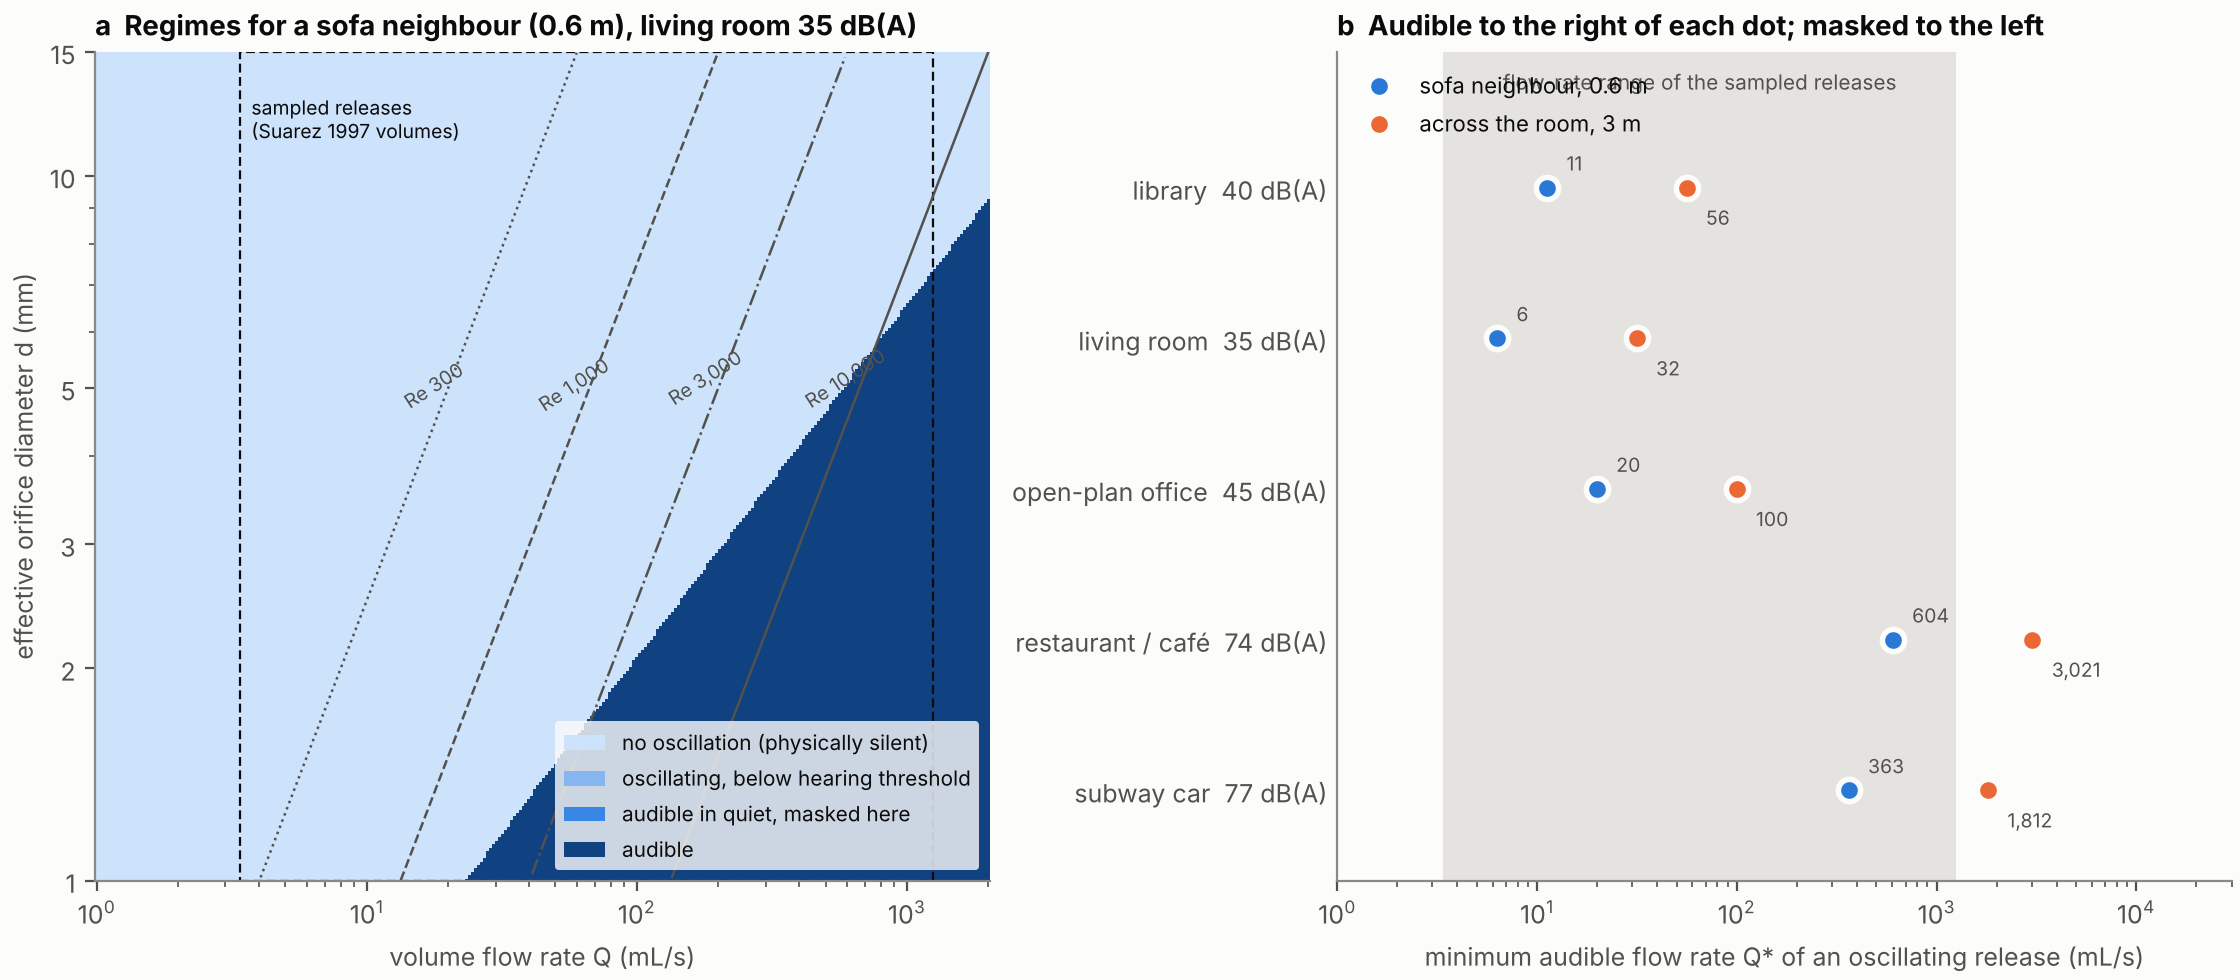
\includegraphics[width=\textwidth]{fig3_acoustic_regimes.png}
\caption{\gap{caption} Acoustic regimes.}
\label{fig:acoustics}
\end{figure}

\subsection{Validation}
\gap{Prose and merged figure (jet + CBL).}

\subsection{The physical ratio}
\gap{Prose.} Equal mass: $R$ = 1.35 (neighbour), 1.73 (own nose). As emitted: 0.92 (neighbour, $P(R>1)$ = 0.47), 1.15
(own nose). Sobol: release volumes explain about 0.6 of the variance as emitted \src{uq/m7\_report.md}.
\begin{figure}
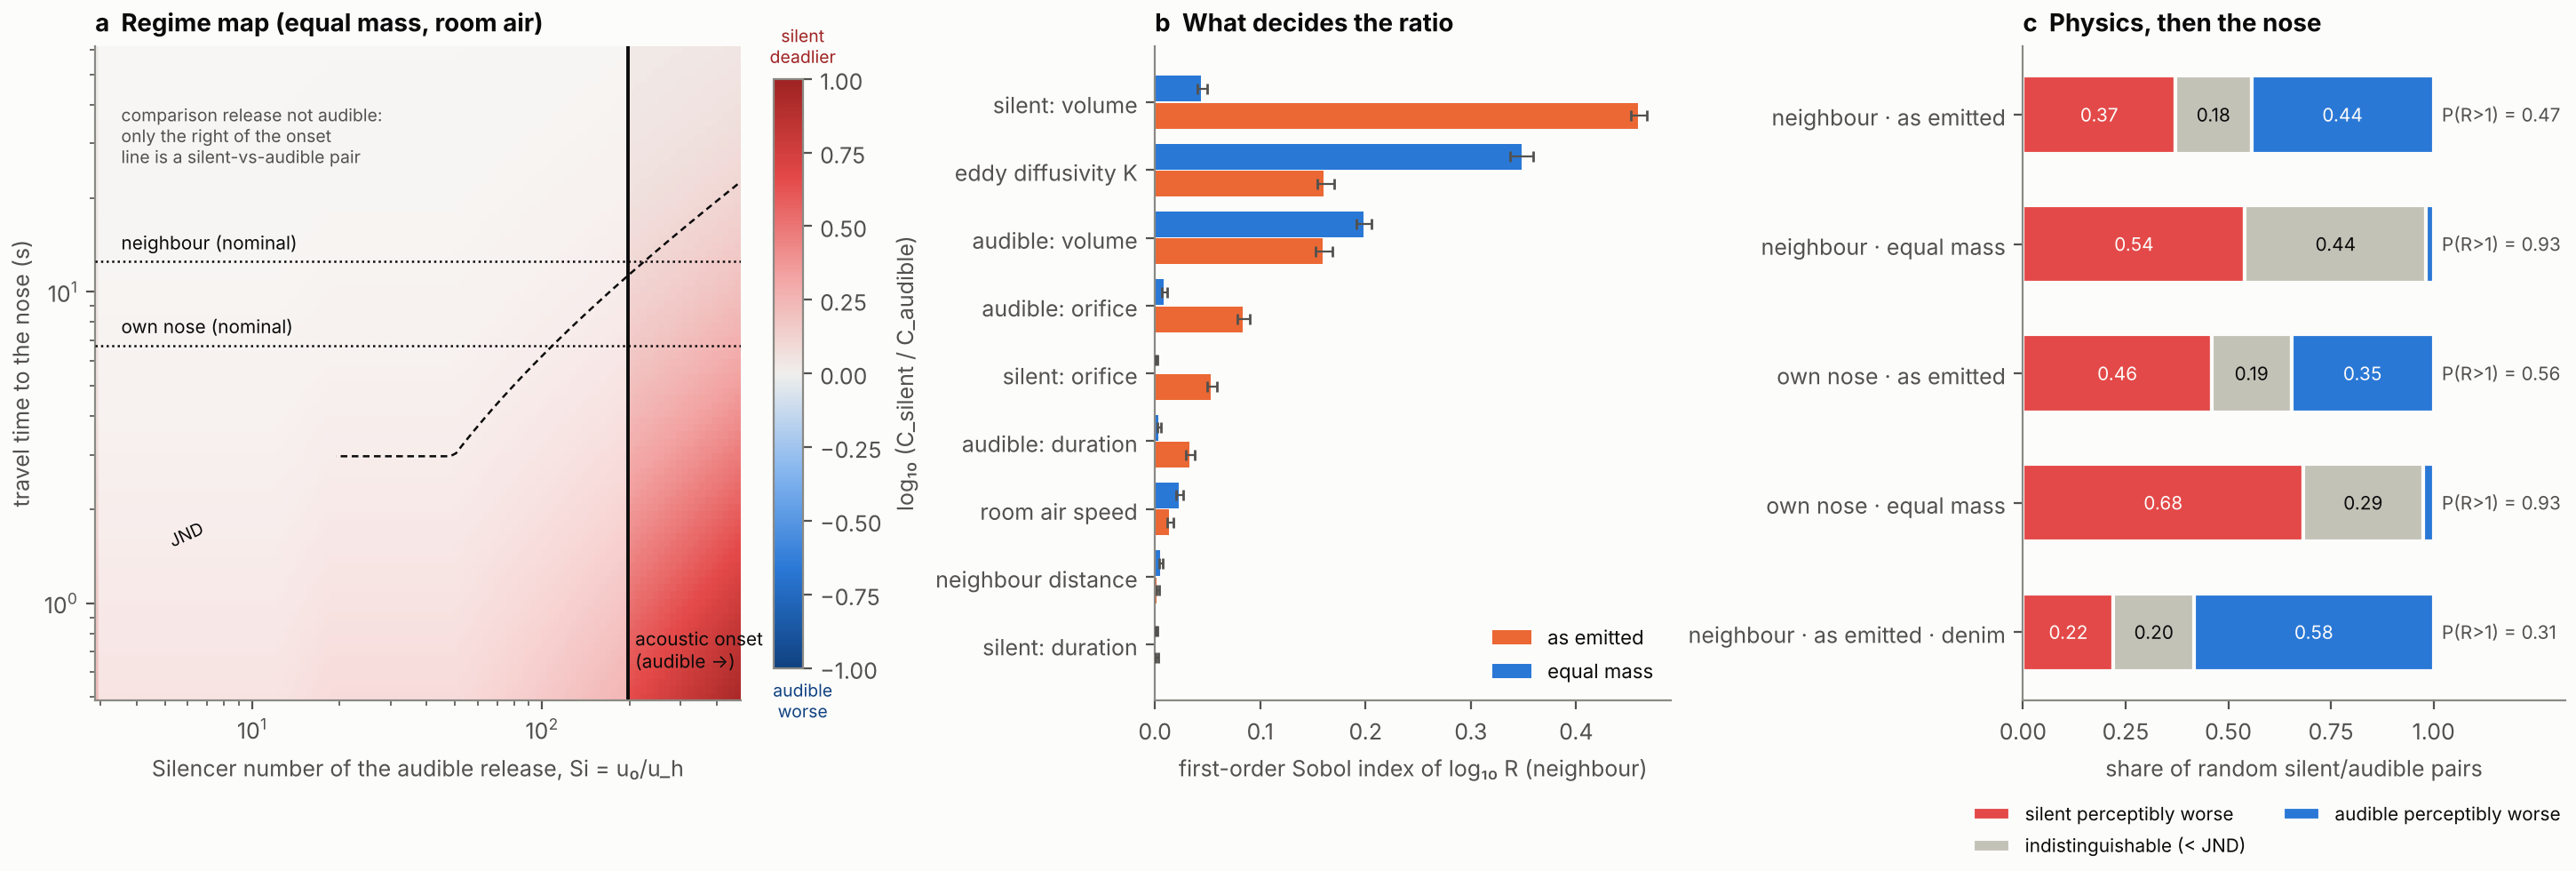
\includegraphics[width=\textwidth]{fig10_regime_uq.png}
\caption{\gap{caption} Regime map, first-order indices and the layered headline.}
\label{fig:uq}
\end{figure}

\subsection{A sofa}
\gap{Prose.} The backrest chimney carries the silent release over the releaser's head; the jet escapes it and reaches the
neighbour \src{cfd/cases/sofa/m4\_report.md}. With the releaser reclined by 4.5\,\textdegree, which closes the back
onto the backrest, the silent release leaves the seat-level wedge sideways and still rises behind the head. No
breathing zone receives a detectable dose. The audible jet now exceeds threshold at the releaser's own nose (OAV 2--4).
In both postures the breathing-zone ratio is $R \approx 10^{-11}$--$10^{-14}$ \src{cfd/cases/sofa/results\_rec4.5.json}.
\begin{figure}
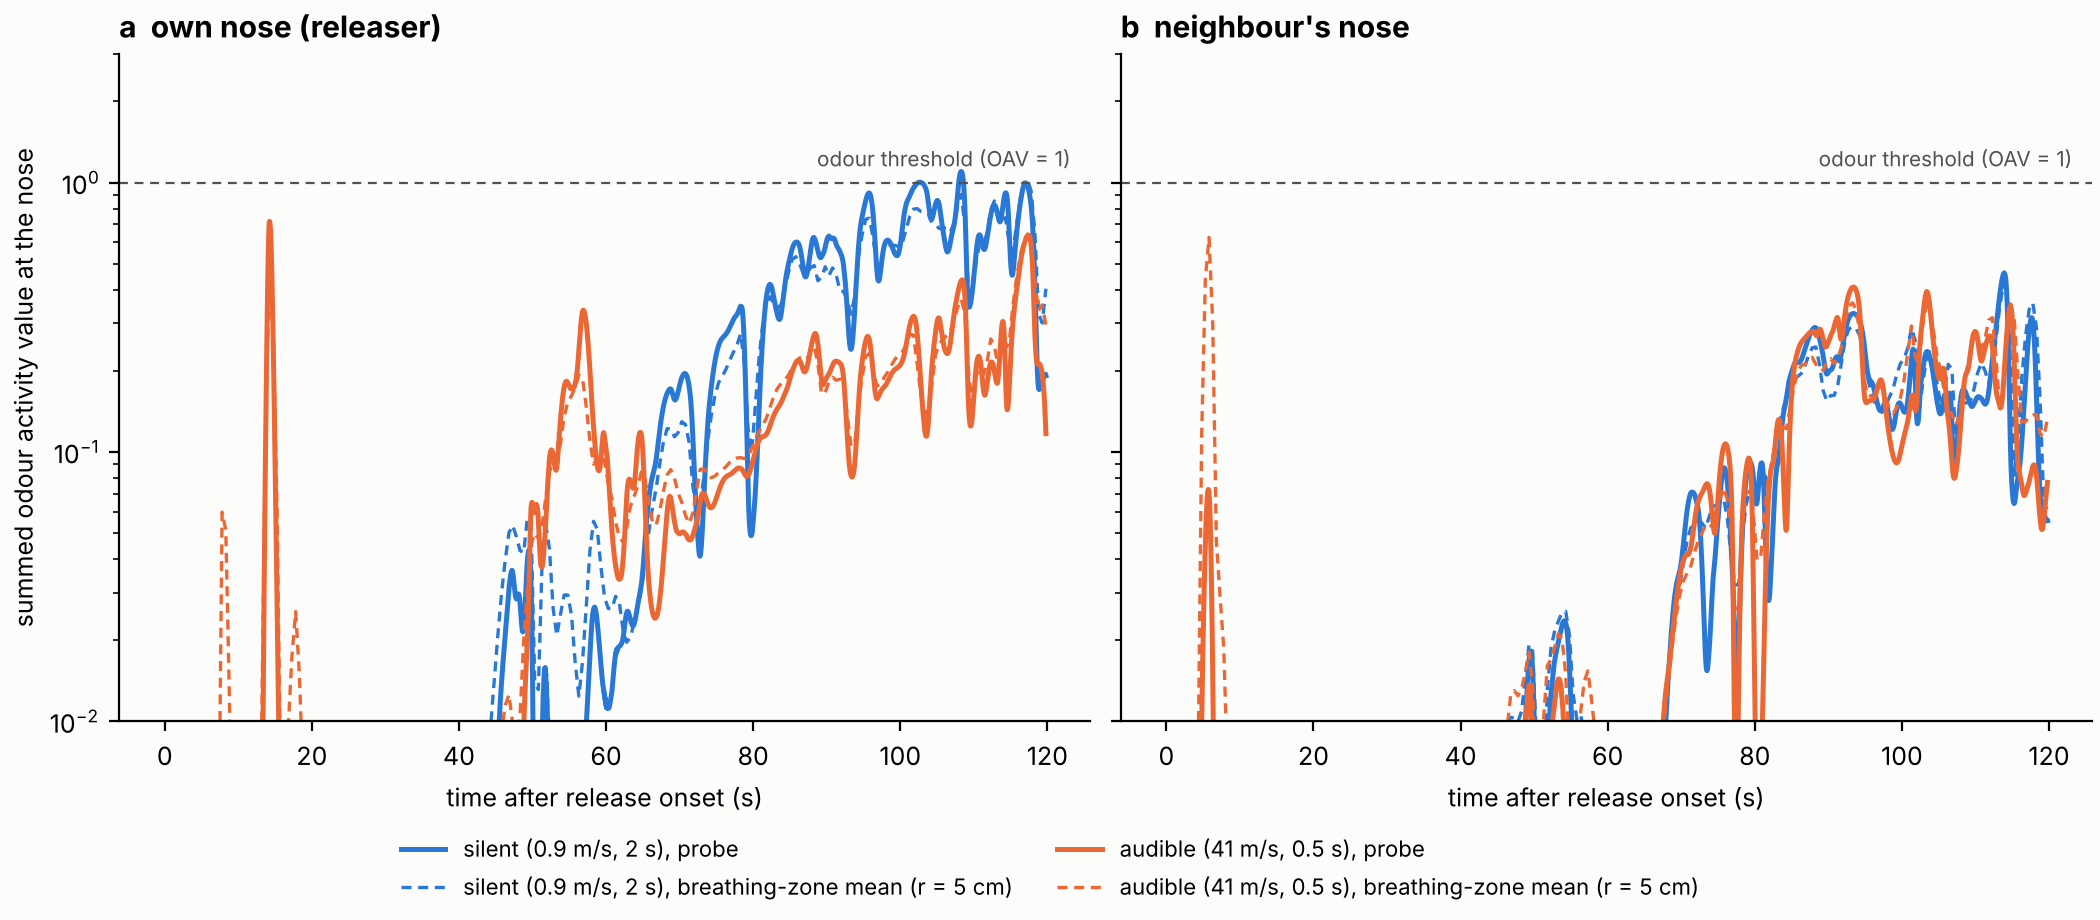
\includegraphics[width=\textwidth]{fig5_sofa_duet_noses.png}
\caption{\gap{caption} Sofa duet: nose time series.}
\label{fig:sofa}
\end{figure}

\subsection{Perception}
\gap{Prose.} Median silent/audible difference at the neighbour: 2.7\% in perceived intensity, below the JND
\src{perception/m6\_report.md}.

\subsection{The composition counter-argument}
\gap{Prose.} No link between passage volume and sulfur concentration; sulfur mass rises with volume
\cite{suarez1997}; nitrogen is blood-derived, not swallowed air \cite{levitt1970,tomlin1991}.

\subsection{Memory}
\gap{Prose.} Truth 0.49; bystander belief 0.67--0.92 across observer models; emitter unbiased
\src{perception/selection.json, uq/observer\_ps.json}.
\begin{figure}
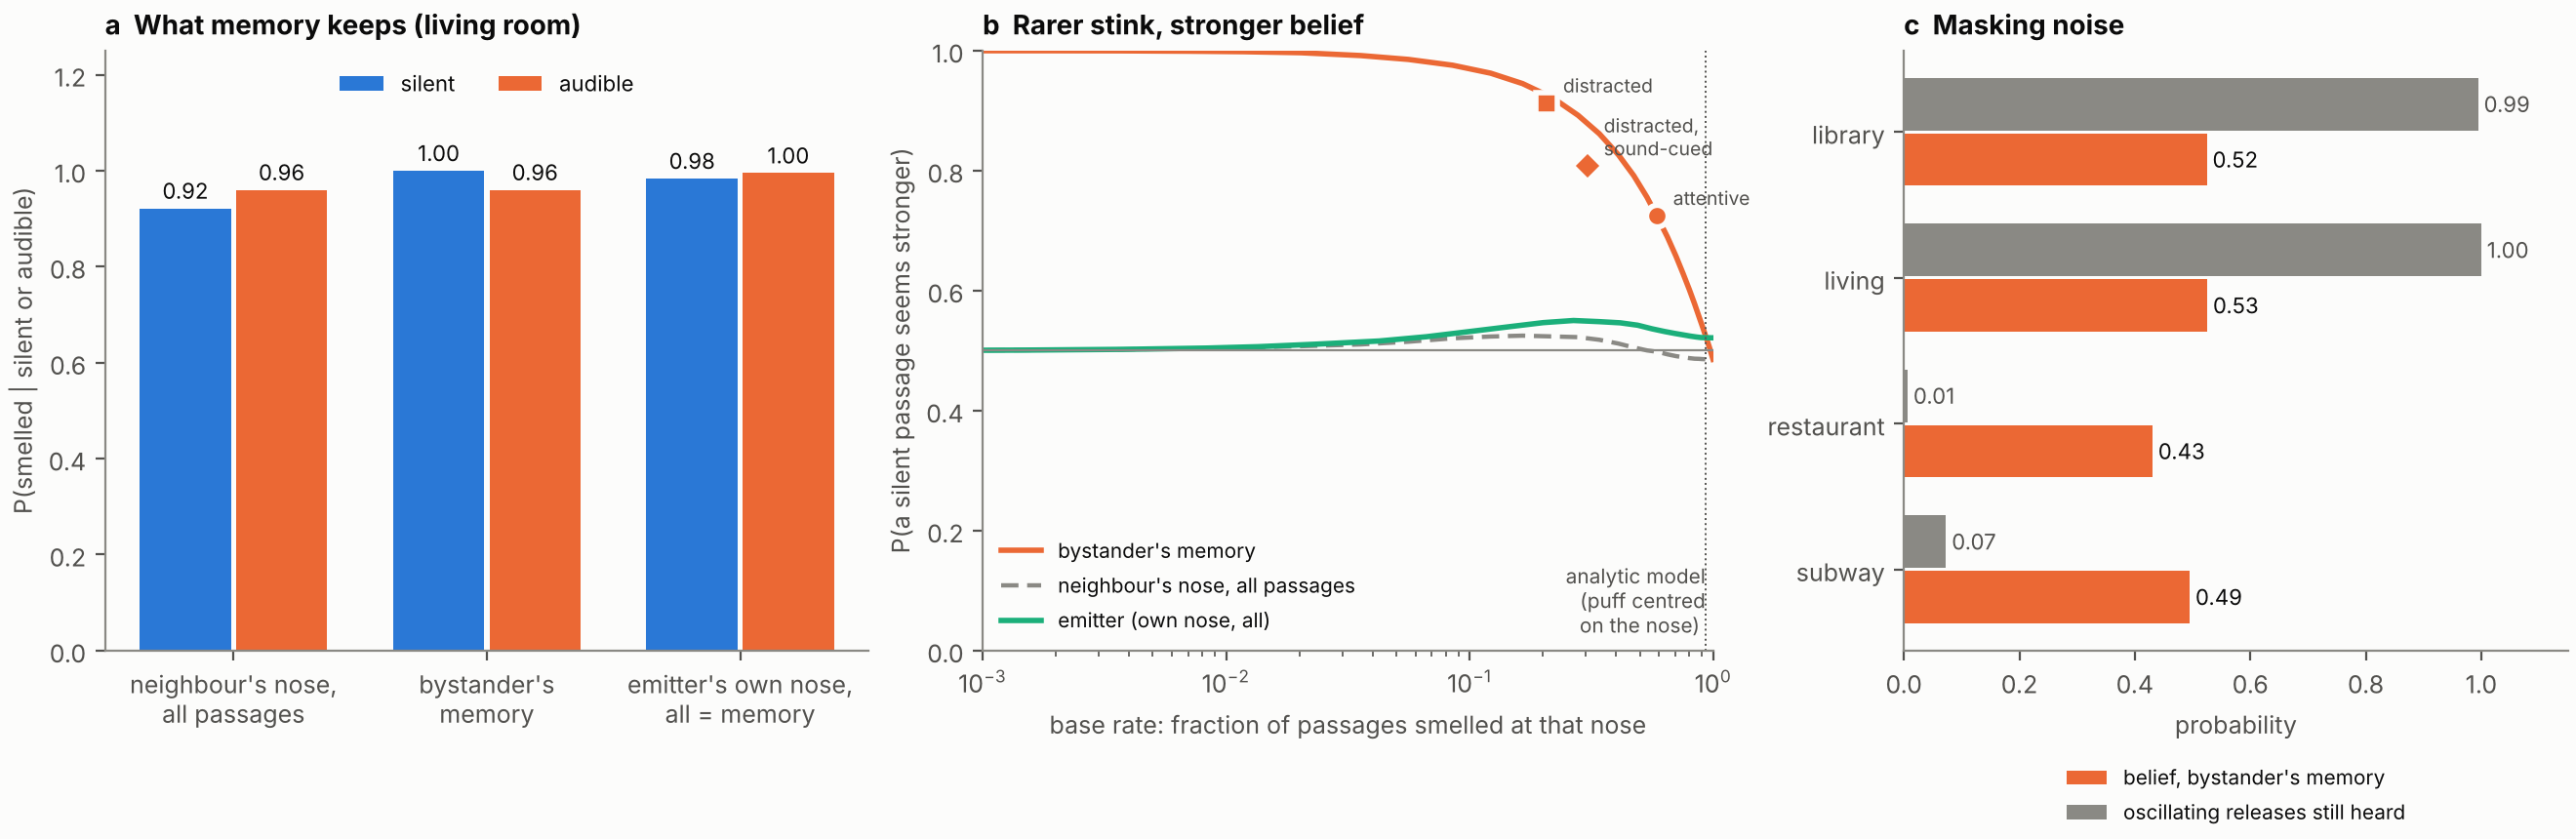
\includegraphics[width=\textwidth]{fig13_memory_filter.png}
\caption{\gap{caption} The memory filter.}
\label{fig:memory}
\end{figure}

\section{Discussion}
\label{sec:discussion}

\subsection{Why the belief exists}
The physics we model does not make silent passages generally worse. At equal mass the silent advantage at a
neighbour is a median factor of 1.35, often below the just-noticeable ratio. As emitted, a silent passage is the
stronger one in 47\% of pairs in the analytic model and in 21\% (0--72\%) of bystander pairs in the simulated scenes,
where on a sofa it misses both noses on its first pass.

The belief is nevertheless documented across languages. Theorem~3 accounts for it without any physical difference: a
passage enters memory if it is heard or smelled, so every remembered silent passage was smelled, whereas audible
passages are remembered whether or not they smelled. With literature observer models this selection turns a truth of
0.32--0.51 into a remembered belief of 0.67--0.92 (Table~\ref{tab:observers}). Three documented memory biases act in
the same direction: distinctive pairings are over-remembered \cite{hamilton1976}, vivid episodes are easy to recall
\cite{tversky1973}, and judgements built from biased samples are rarely corrected \cite{fiedler2000,denrell2005}. The
phrase itself can also pass the belief on without any experience \cite{chapman1967}; documentary evidence cannot
separate the two routes (Figure~\ref{SI-fig:culture}).

\subsection{The releaser}
The releaser feels every release, so their noticing does not depend on smell and Theorem~3 does not apply to them.
Three findings bear on how they judge their own passages.
\begin{itemize}
  \item People rate their own flatus as less disgusting than a stranger's: on a 1--5 scale the item ``silent but
  smells strongly'' is rated 2.51 for one's own flatus and 3.71 for a stranger's \cite{liuzza2016,stevenson2005}.
  This lowers the unpleasantness of the releaser's own passages, not the contrast between silent and audible ones.
  \item The self-advantage appears even when people do not recognise their own odour \cite{mcburney1976}.
  \item Believing an odour is one's own shifts its hedonic rating \cite{hold1977}, so expectation is the one route by
  which a releaser could share the belief.
\end{itemize}

\subsection{Where the odour comes from}
\label{sec:disc-chem}
Two facts the transport model takes as given have chemical explanations in the literature; we did not test them.

\emph{Why sulfur concentration does not follow volume.}
\begin{itemize}
  \item \ce{H2S} comes from sulfate-reducing bacteria and from cysteine degradation, whose genes are widespread in the
  gut microbiome \cite{gibson1993,braccia2021}. Sulfate reducers outcompete methanogens for \ce{H2} by affinity
  ($K_s \approx 1$ against 6\,\textmu mol\,L$^{-1}$), and sulfide and methane production tend to exclude each other
  \cite{gibson1993}.
  \item The caecal mucosa of rats removes both gases quickly: methanethiol is demethylated to \ce{H2S}, and \ce{H2S} is
  oxidised mainly to thiosulfate \cite{levitt1999}. Rhodanese is the main detoxifying enzyme in human colon
  \cite{picton2002}, and SELENBP1 oxidises methanethiol with an apparent $K_m$ of 4.8\,nM \cite{pol2018}.
  \item Only free sulfide can enter the gas, and it is less than 5\% of faecal total sulfide \cite{tangerman2009}.
\end{itemize}
The odorants are thus trace products held at a balance of production and fast consumption, whereas passage volume is
set by \ce{N2}, \ce{CO2}, \ce{H2} and \ce{CH4}. We infer that this is why sulfur concentration and passage volume are
uncorrelated \cite{suarez1997}. Diet moves the balance: a meat-rich diet raised faecal sulfide from 0.22 to
3.38\,mmol\,kg$^{-1}$ in five volunteers \cite{magee2000}, and the response to animal and plant diets differs between
people \cite{teigen2022}.

\emph{Why methanethiol smells foul.} The human receptor OR2T11 responds to short thiols, including methanethiol, in a
copper-dependent way, but not to \ce{H2S} \cite{li2016}. Human nasal mucus contains about 2.5\,\textmu M copper
\cite{block2017}, below the 30\,\textmu M added in the receptor assays, so the receptor's role in vivo is plausible
but not shown. Other receptors respond to sulfur ligands without copper \cite{duan2012,haag2019,zhang2018}. A
receptor that responds to methanethiol and not to \ce{H2S} would make methanethiol the characteristic note of flatus
independently of thresholds; we infer this, it has not been tested.

\subsection{Predictions}
Theorem~3 predicts that releasers hold the belief less firmly than bystanders and that people without a sense of
smell never remember a silent passage. Because masking removes the quieter audible passages, the effect of background
noise on the belief should be ambiguous.

\subsection{When a silent release is worse}
At equal mass, at the releaser's own nose, in still air and within a few seconds, a silent release is perceptibly
stronger than a loud one (Figure~\ref{fig:uq}a). In the elevator, a silent release is also stronger for the person
standing behind a front-row releaser, who smells it first. In these two cases the saying holds.

\subsection{Limitations}
\begin{itemize}
  \item \emph{Mean flow only.} The CFD resolves the mean flow; instantaneous peaks of a meandering cloud can exceed the
  mean by an order of magnitude. This can lift the sub-threshold audible doses on the sofa (OAV 0.2--0.6) above
  threshold, but not the silent ones ($10^{-10}$). In the forward-leaning posture the mean silent cloud passes within
  25\,cm of the neighbour's face, where a filament could reach the nose.
  \item \emph{Body plume.} The seated body plume is 40--56\% too fast, which shortens the travel times of the silent
  release by about 30\% in the seated case; the arrival times in the elevator (8.8 and 17.6\,s) are likely short by a
  similar amount. Standing plumes were not validated separately.
  \item \emph{Scenes and weights.} The as-emitted shares of Figure~\ref{fig:routing} weight the simulated scenes
  equally and assume the flow path does not depend on the passage volume. They describe these scenes, not how often
  each arises.
  \item \emph{Base rate.} The share of passages smelled has never been measured; the remembered belief of
  0.67--0.92 spans the observer models that bracket it.
\end{itemize}

\section{Conclusion}
\label{sec:conclusion}

\begin{itemize}
  \item \emph{Routing.} The body's convective boundary layer takes a slow release and lets a fast one pass, so the
  momentum of a release next to a body decides which nose it reaches. On a sofa the silent release rises behind the
  releaser to the ceiling and misses both noses on its first pass; in an elevator it is strongest for the person
  standing behind the releaser. \gap{v4: standing pair}
  \item \emph{Peak bound.} Under linear transport a slower release of the same gas never gives a higher peak, in any
  room or flow. Only the near-field pre-dilution of a fast jet lets a silent release win: by a median factor of 1.45
  at equal mass in the analytic model, often below the just-noticeable ratio. As emitted, a silent passage is the
  stronger one at the neighbour in 48\% of pairs in the analytic model and at a bystander in \gap{v4; preprint: 21\%
  (0--70\%)} of pairs in the simulated scenes.
  \item \emph{Selection.} A silent passage is noticed only if it is smelled, and this selection alone can explain the
  belief: in literature observer models a remembered silent passage seems the stronger one in \gap{v4; preprint:
  68--93\%} of comparisons. The explanation predicts that releasers hold the belief less firmly than bystanders and
  that people without a sense of smell never remember a silent passage.
\end{itemize}


\begin{acknowledgement}
\gap{AI-use disclosure, required by arXiv and ACS policy: Claude Code (Anthropic) wrote code, ran simulations,
searched and extracted literature and drafted text; the author reviewed all content and takes responsibility.
To be written last, per the author.}
\end{acknowledgement}

\begin{suppinfo}
Overview diagram; CFD validation; the CFD scenes in detail (sofa postures, elevator, standing pair); breath
sampling; the cross-cultural survey; source files of every result; and the full parameter table (PDF). Code and data:
\gap{Zenodo DOI}.
\end{suppinfo}

\bibliography{refs}

\end{document}
